\chapter{Les outils}       
Les outils occupent une part importante du stage.
L'équipe de Mimesis Republic est à la pointe de la technologie et utilise de
nombreux outils pour accélérer le développement.\\
La plupart de ces outils sont open source, un certain nombre sont assez jeunes
et rarement utilisés par les entreprises en général, qui ne prennent
probablement pas le risque de s'engager avec des nouveaux outils.\\ 
Ceux-ci demandent effectivement un effort d'apprentissage et d'adaptation au
début mais une fois maîtrisés, le gain de productivité est réel.\\

Je décris ci dessous chacun de ces outils,
classés par temps d'utilisation dans le travail que j'ai effectué.
Les outils que j'ai le plus utilisés sont présentés en premier et sont décrits
de façon plus complète, avec leurs avantages et inconvénients.

\section{Scala}
Scala est le langage de programmation utilisé pour développer l'univers \textit{Mamba
  Nation}.\\
Le moteur 3D du jeu est codé en Scala, les mécaniques de gameplay sont codés en
Scala,\\
l'outil d'infrastructure coté serveur est aussi codé en Scala.

C'est un langage de programmation multi-paradigme conçu à l'École Polytechnique
Fédérale de Lausanne (EPFL).
Son nom vient de l'anglais Scalable language qui signifie  ``langage évolutif''
. 

\subsection{Caractéristiques et points forts de Scala}

\begin{itemize}
\item[\textbullet]\textbf{Tourne sur la JVM :}\\
  Il est prévu pour être compilé en bytecode Java (exécutable sur la JVM).
  Il existe aussi un portage sur la machine virtuel .Net qui reste néanmoins
  moins abouti que pour la JVM.\\

  Si on souhaite utiliser Scala exclusivement avec la JVM, il est alors possible
  d'utiliser les bibliothèques écrites en Java de façon complètement
  transparente. Ainsi, Scala bénéficie de la maturité et de la diversité des
  bibliothèques qui ont fait la force de Java depuis une dizaine d'années.\\

\item[\textbullet]\textbf{Tout dans les bibliothèques :}\\
  Le coeur du langage est minimal, la plupart des fonctionnalités majeures se
  trouvent être implémentées dans des bibliothèques.\\
  C'est un point important pour l'évolutivité du langage.\\

  Un exemple : les collections standards Scala sont faciles à utiliser, concises
  et semblent faire partie du langage même si elles sont en fait implémentées
  dans une bibliothèque.\\
  Quelques lignes suffisent pour partitionner une liste \textit{people} en deux
  autres (\textit{minors} et \textit{adults}), en fonction de leur age :
\lstset{language=Scala}
\begin{lstlisting}
    class Person(val name:String, val age:Int)
    val people = List(
    new Person("Hervé", 22),
    new Person("Julie", 17),
    new Person("Greg", 18))

    val (minors, adults) = people partition (_.age < 18)
\end{lstlisting}

Ce morceau de code demanderait plusieurs boucles imbriquées en Java.\\
Ici, List est juste une classe et partition une méthode.\\
Ces fonctionnalités étant toutes implémentées dans des bibliothèques,
le programmeur peut lui aussi écrire ses propres bibliothèques qui seront
faciles d'utilisation, concises et extensibles.\\

\item[\textbullet]\textbf{Orienté objet pur :}
  \begin{itemize}
  \item Toute valeur est un objet \\
    1.hashCode renvoie 1
  \item Toute opération est un appel de méthode :\\
    le compilateur remplace 1 + 2 par (1) .+ (2)\\
  \end{itemize}
  Les exceptions à ces règles de Java ont été supprimées :\\
  Plus de primitives comme int, float (Int et Float à la place).\\
  Plus de qualificateur ``static'' mais un mot clef ``object'' qui équivaut à créer
  automatiquement un singleton thread safe en Scala. \\
  Ces quelques changements contribuent à rendre le langage plus extensible
  que Java.\\
\item[\textbullet]\textbf{Fonctionnel :}\\ 
  Toutes les fonctions sont des valeurs et puisque toute valeur est objet en
  Scala, toute fonction est aussi un objet. 
  Scala offre une syntaxe légère pour les fonctions anonymes, supporte les
  fonctions de premier ordre, possède les case classes et le pattern matching.\\
  Par contre la récursion terminale n'est pas complètement supportée à cause du
  manque de support de la JVM pour la récursion terminale. Le compilateur Scala
  optimise les cas simples d'appels terminaux en boucle while.\\
\item[\textbullet]\textbf{Statiquement typé :}\\
  Scala est un langage fortement typé qui permet d'assurer une certaine sécurité
  dans les programmes, offrir de bonnes performances (aujourd'hui les langages
  statiquement typés ont tendance à être plus rapides que les langages
  dynamiquement typés) et facilite le refactoring de code car de nombreuses
  erreurs sont signalées par le compilateur lorsque un changement est effectué.\\
\item[\textbullet]\textbf{Inférence de types :}\\
  Les types ne doivent pas être nécessairement indiqués car ils peuvent être
  inférés automatiquement par le compilateur dans la majorité des cas.\\
  Le code source est plus aéré et le développeur n'a pas à se soucier de retenir les
  noms de types.
  L'indication des types reste toutefois obligatoire pour les paramètres de
  méthodes.\\
\item[\textbullet]\textbf{Autorise la Surcharge d'opérateurs :}\\
  Tout opérateur est une fonction. Une surcharge d'opérateur n'est rien d'autre
  qu'une surcharge de méthode en Scala.\\
\item[\textbullet]\textbf{Possède un interpréteur en ligne de commande :}\\ 
  Comme python et son ipython, Scala possède un environnement de programmation
  interactif en ligne de commande (REPL, read-eval-print-loop).\\
  Le REPL facilite grandement l'apprentissage d'un nouveau langage puisqu'il
  donne de rapides retours sur le code entré.\\
\item[\textbullet]\textbf{Trait :}\\Entre les interfaces Java et l'héritage
  multiple C++, les traits peuvent avoir des implémentations de méthode et des
  champs tout en rendant impossible l'héritage en diamant.\\
  Ruby est un autre langage qui possède les traits.\\  
\item[\textbullet]\textbf{Performant :}\\Les performances de Scala sont comparables
  à celles de Java. Le paradigme fonctionnel de Scala incite à utiliser des
  données immuables et favorise l'activation de certaines optimisations de la
  JVM.\\
  Papier publié par Google qui compare les performances de Java, C++, Go et Scala :
  \url{https://days2011.scala-lang.org/sites/days2011/files/ws3-1-Hundt.pdf}\\
\end{itemize}


La principale caractéristique qui rend le langage évolutif reste que Scala
fusionne les paradigmes fonctionnel et orienté objet à merveille, bien plus loin
que n'importe quel autre langage.\\
Je pense en particulier aux programmeurs OCaml qui peuvent, à souhait, utiliser
la programmation fonctionnel ou objet mais qui dans 90\% des cas d'utilisations
utilisent le coté fonctionnel du langage.\\
En Scala, la mixité entre les deux paradigmes est réelle avec une utilisation
légèrement supérieure de l'orienté objet (estimation grossière : 60\% objet, 40\%
fonctionnel).\\

Les paradigmes fonctionnel et orienté objet sont fondamentalement différents
et chacun possède des caractéristiques qui facilitent la résolution d'un type
de problème.\\
La complémentarité des paradigmes fonctionnel et orienté objet :\\\\
\begin{tabular}{|c|c|}
  \hline
  \textbf{fonctionnel} & \textbf{orienté objet}\\
  \hline
  Facilite la production de code simple & Facilite l'adaptation et l'extensibilité\\
  grâce aux fonctions de premier ordre, & de projets complexes grâce aux\\
  closures, et pattern matching & classes, sous typage et héritage \\
  \hline
\end{tabular}


\subsection{Faiblesses du langage}
\begin{itemize}
\item[\textbullet] Bien que le langage soit aujourd'hui mature et prêt à être utilisé en
  entreprise, peu ont fait le pas.\\
  Toutefois, quelques entreprises bien connus utilisent aujourd'hui Scala.
  C'est le cas de Twitter, LinkedIn et Foursquare qui ont incorporés Scala au
  cœur de leurs projets.\\
  Par exemple Twitter a transféré tout leur code coté serveur de Ruby en Scala,
  afin d'avoir les meilleurs performances possibles tout en gardant un langage
  extensible pouvant faire face à l'évolution croissante de leurs demandes.\\

  Néanmoins, Scala reste pour l'instant un langage de niche avec une estimation
  de 0.237\% d'utilisation pour le mois de juillet 2012 calculée par le site
  \href{http://www.tiobe.com/index.php/content/paperinfo/tpci/index.html}{tiobe.com}.\\
\item[\textbullet] Les plugins IDE Scala progressent lentement et restent
  faibles en fonctionnalités comparés à ce qu'offrent les IDE Java.\\
\item[\textbullet] Le compilateur du langage, Scalac, est lent
  (approximativement 10 fois plus lent que javac pour un nombre de lignes de
  code équivalent)\\
\end{itemize}

Pour finir cette présentation du langage, voici deux citations de deux
créateurs de langages :\\
\textbf{James Gosling}, créateur de Java :\\
``If I were to pick a language to use today other than Java, it would be
Scala.''\\\\
\textbf{James Strachan}, créateur de Groovy :\\
``I can honestly say if someone had shown me the Programming in Scala
book by Martin Odersky, Lex Spoon and Bill Venners back in 2003 I’d probably
have never created Groovy.''\\


%% ne pas utiliser l'indentation automatique sinon ça va décaler le code sur la
%% droite et ça ne tiendra pas sur le pdf
\clearpage
Équivalences de code Java, Scala :\\
\noindent
\small\addtolength{\tabcolsep}{-5pt}
\begin{tabular}{|c|c|}
  \hline
  \textbf{Java} & \textbf{Scala}\\
  \hline
  \lstset{language=Java}
  \begin{lstlisting}
boolean hasUpperCase = false
for (int i = 0; i < name.length(); i++)
  if (Character.isUpperCase(name.charAt(i))) {
    hasUpperCase = true;
    break;
  }
\end{lstlisting} &   \lstset{language=Scala}
\begin{lstlisting}
// Utilisation des collections et closures Scala
val hasUpperCase = name.exists(_.isUpper)
\end{lstlisting}
\\
\hline
\lstset{language=Java}
\begin{lstlisting}
public class Person {
  private String name;
  private int age;
  public Person(String name, int age) {
    this.name = name; this.age = age;
  }

  public String getName() { return name;}
  public int getAge() { return age; }

  public void setName(String name) { 
    this.name = name; 
  }
  public void setAge(int age) { 
     this.age = age; 
  }
}
\end{lstlisting} &
\lstset{language=Scala}
\begin{lstlisting}
// Scala créé automatiquement les getters et
// setters pour 'name' et 'age'
class Person(var name: String, var age: Int)
\end{lstlisting}
\\
\hline
\end{tabular}


\section{Play!}

Play! est un framework MVC inspiré de Rails qui permet de créer facilement des
applications web avec Java et Scala.

%% Play est basé sur une architecture légère et stateless avec une consommation de
%% ressources (CPU, mémoire, threads) minimale pour les applications évolutives.

\subsection{Full stack}
Play! embarque un serveur web, il se suffit à lui-même. Cette notion
est appelée “full-stack”. Elle signifie que Play! est autonome 
dans son mode de développement en proposant tout ce qu’il faut pour faire
une application web, de la couche présentation à l’accès aux données.
En production, les applications Play! s'exécutent grâce au serveur web intégré.

\subsection{Choix libre de la technologie coté client}

Le framework Play! ne s’occupe que de la partie coté serveur.
Coté client, nous avons le choix des technologies (HTML5 + CSS3 + jQuery
par exemple).

Play! offre un support natif pour deux technologies clientes :
CoffeeScript et LESS.
\begin{itemize}
\item CoffeeScript est un petit langage qui compile vers du JavaScript.
  Il propose une syntaxe concise et permet d'éviter les nombreux pièges de
  JavaScript. Il y a une relation 1-1 entre du code JavaScript et du code
  CoffeeScript.
\item LESS est un petit langage lui aussi mais qui compile vers du CSS.
  Grâce à LESS, il est possible de rajouter des variables, des opérations
  (comme additionner des couleurs ensemble) et faire de l'héritage dans nos
  fichiers de styles.
\end{itemize}

\bigskip

CoffeeScript a été utilisé pour le développement du projet mais le besoin
d'utiliser LESS ne s'est pas fait sentir.

\subsection{Architecture stateless}

Play! est stateless, le serveur n'a aucune vision du client.
Il n'existe pas d'état (session) côté serveur, l'état est stocké coté client (dans
des cookies et cache) et/ou en BDD.
\bigskip

C'est la requête qui ``porte'' toutes les informations nécessaires à l'exécution
de l'action :\\
http://monsite/donne/moi/utilisateur/12 \\
Le serveur reçoit une requête, traite la requête puis renvoie une réponse.
Après envoie de la réponse, le client est oublié.

Dans une architecture stateful, l'historique d'activité du client sur le site
web va être conservé coté serveur (il est allé sur tel page, puis il a cliqué tel
bouton) alors que dans une architecture stateless, cette information n'est pas
gardée.

Une architecture stateless permet d'avoir de meilleurs performances et une
faible consommation mémoire. Play! offre de bonnes performances car les requêtes
peuvent être traîtées : 
\begin{itemize}
\item dans le désordre
\item par 2 (ou+) serveurs différents
\end{itemize}
et Play! consomme peu de mémoire car :
\begin{itemize}
\item il n'y a pas de session sauvegardée coté serveur
\item il n'y a pas de réplication de session
\end{itemize}

\subsection{Rechargement à chaud et affichage des erreurs dans le navigateur}

\begin{figure}[H]
  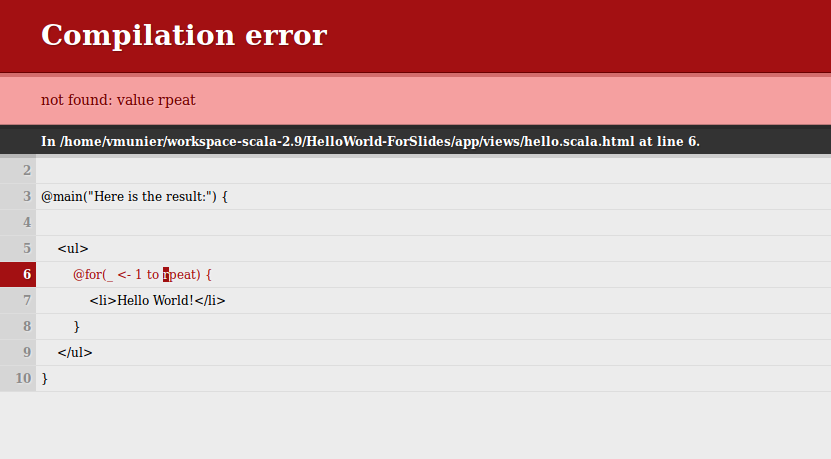
\includegraphics[scale=0.40]{play-erreur.png}  
\end{figure}

Le cycle de développement est rapide, edition $\rightarrow$ test $\rightarrow$ correction.
Avec Play! il y a un seul endroit où consulter le résultat de son
application : le navigateur. 

Avec des frameworks web Java classiques (JSF par exemple), une erreur peut se
produire à plein d'endroits différents :
\begin{itemize}
\item Est-ce qu'il faut regarder dans son Eclipse pour trouver une erreur de
  compilation ?
\item Est-ce qu'il faut regarder dans son navigateur pour trouver une erreur de
  rendu ?
\item Est-ce qu'il faut regarder dans sa console pour trouver une erreur à
  l'exécution et chercher la ligne qui nous intéresse dans une stacktrace
  gigantesque ? 
\end{itemize}

\bigskip

Le cycle de développement est plus simple avec Play!.
On édite le code dans son éditeur de texte, on sauvegarde et enfin on rafraîchit
la page dans son navigateur et c'est dans son navigateur qu'on vérifie si il n'y
a pas d'erreur. \\
Bien sur, nous pouvons aussi utiliser notre IDE favori et avoir le
surlignement des ereurs mais un simple éditeur de texte suffit pour développer
avec Play! (TextMate, Vim, Emacs).

\section{Simple Build Tool (SBT)}

SBT est un outil de build écrit en Scala et configurable en Scala.
C'est l'équivalent de Maven.  

Les fichiers de configurations SBT sont moins verbeux que leurs fichiers POM
équivalents. Ils sont écrits en Scala et peuvent donc profiter de toute la
puissance du langage pour exprimer n'importe quel besoin. Par exemple, 
la commande \textit{compile} peut être surchargée pour générer des fichiers sources avant
que l'étape de compilation suive.

\section{Amazon Web Services (AWS)}

Amazon Web Services (AWS) est une collection de services informatiques distants
 fournis via internet par Amazon.com.

\subsection{Elastic Compute Cloud (EC2)}

Son service le plus populaire est l'Amazon Elastic Compute Cloud ou EC2 qui
permet à des tiers de louer des serveurs sur lesquels exécuter leurs propres
applications web. EC2 permet un déploiement extensible des applications en
fournissant une interface web par laquelle un client peut créer des machines
virtuelles, c'est-à-dire des instances du serveur, sur lesquelles le client peut
charger n'importe quel logiciel de son choix. Un client peut créer, lancer, et
arrêter des instances de serveurs en fonction de ses besoins, et paye en
fonction du temps d'usage des serveurs d'où le terme de « Elastique ».

Informations reprises de wikipedia :
\href{http://fr.wikipedia.org/wiki/Amazon_Elastic_Compute_Cloud}{EC2 Wikipedia}\\

\subsection{Relational Database Service (RDS)}

Amazon propose aussi un service pour gérer sa Base de données (Amazon
Relational Database Service (RDS)). 
RDS facilite l'installation, l'exploitation et le dimensionnement d'une base de
données relationnelle dans le nuage. La capacité de la BDD est redimensionnable.
MySQL, Oracle et Microsoft SQL Server sont supportés.

\subsection{Route 53}

Amazon permet aussi de personnaliser et contrôler ses ressources réseau dans le
nuage.
Route 53 est un service Web de système de noms de domaine (DNS) hautement
disponible et évolutif. C'est sur Route 53 que nous définissons les couples
URL/adresses IP pour acheminer les utilisateurs finaux vers une application
web.

\section{Chef}

Administrer un seul serveur est une tâche assez simple. Administrer un parc de
serveurs est déjà beaucoup plus difficile et la tâche devient extrêmement
complexe quand les systèmes sont hétérogènes, c'est à dire lorsque nous avons
des systèmes différents Unix, Linux et Windows (ce qui sera toujours le cas au
bout de quelques années au moins).\\

Imaginons que nous voulions changer l'IP de nos serveurs DNS, il nous faudra
alors se connecter sur chaque serveur pour modifier le fichier
/etc/resolv.conf. Il en est de même pour vérifier les droits de certains
fichiers critiques, pour s'assurer qu'un programme est lancé sur tels
serveurs.\\

Pour répondre à ces problèmes qui ont occupé et occupent toujours des bataillons
d'administrateurs système, il existe trois acteurs majoritaires sur le marché
qui sont : Puppet, Chef et Cfengine. Chef est le plus jeune des trois. 

Avec sa DSL (Domain-Specific Language) ruby, Chef réalise une abstraction
d'opérations de base comme la manipulation des IPs, de la configuration DNS ou
NTP, etc. \\
Un de ses points forts est que la même fonction Chef permet de manipuler des
choses décrites différemment selon le système : une IP ne s'affecte pas de la
même façon sous Linux que Solaris ou Windows.\\
L'administrateur système décrit son infrastructure avec la DSL ruby et Chef
se charge de maintenir dans le temps la cohérence de cette infrastructure.


%% \section{Eclipse}

%% Un plugin Scala pour la coloration syntaxique, complétion de code et débugger
%% intégré est disponible sous Eclipse.\\
%% Les fonctionnalités disponibles dans Eclipse pour le langage Java
%% restent toutefois bien supérieures à celles proposées pour Scala qui ne possède
%% pas encore d'importation automatique de packages ou de context assist.\\

%% Cependant, Scala tourne sur la JVM et peut profiter de nombreux outils bien
%% intégrés dans Eclipse qui étaient destinés originalement au langage Java.\\
%% Par exemple FindBugs et JavaRebel sont tout aussi fonctionnel avec Scala.

\section{Jira}

%% Les "workflow" de Jira
%% https://confluence.atlassian.com/display/JIRA/Configuring+Workflow

C'est un logiciel de gestion de projet qui se présente sous forme de page web
accessible depuis internet.

Le chef de projet crée des Issues qu'il met en ligne dans Jira.
Une issue, identifiée par un numéro unique, est la description d'une
fonctionnalité à ajouter ou d'un bug à corriger. 
Cette description de l'issue contient notamment :
\begin{itemize}
\item la date de création de l'issue
\item la priorité de l'issue (Must, Should, Would, Could)
\item le nombre d'heures estimé pour réaliser la tâche
\item le nombre d'heures restant
\item le nombre d'heures loguées
\item l'historique des modifications apportées à cette issue.\\

\end{itemize}

Chaque membre de l'équipe peut laisser un commentaire sur l'issue pour
proposer des idées de solution.\\

\textbf{Avantages} :
Les objectifs voulus sont clairs, ils sont définis et notés dans une issue.
De fait, lorsque l'auteur poste une issue, il a réfléchi à la demande avant de
l'écrire. \\
Une pratique de quelques chefs de projet est de faire les demandes à l'oral.
Une demande orale est bien moins utile qu'une demande écrite car le chef de
projet oublie facilement des détails et se trouve être moins précis que s'il
avait pris le temps de choisir les bonnes phrases dans une demande écrite.\\
Quant au développeur, avoir une demande écrite lui permet de l'analyser
ultérieurement.


\subsection{Le workflow de Jira}

Un workflow Jira est un ensemble d'étapes (ou d'états) et de transitions qu'une
issue traverse durant son cycle de vie. Les workflows Jira sont consistitués
d'étapes et de transitions.

\begin{wrapfigure}[13]{r}{11cm}
  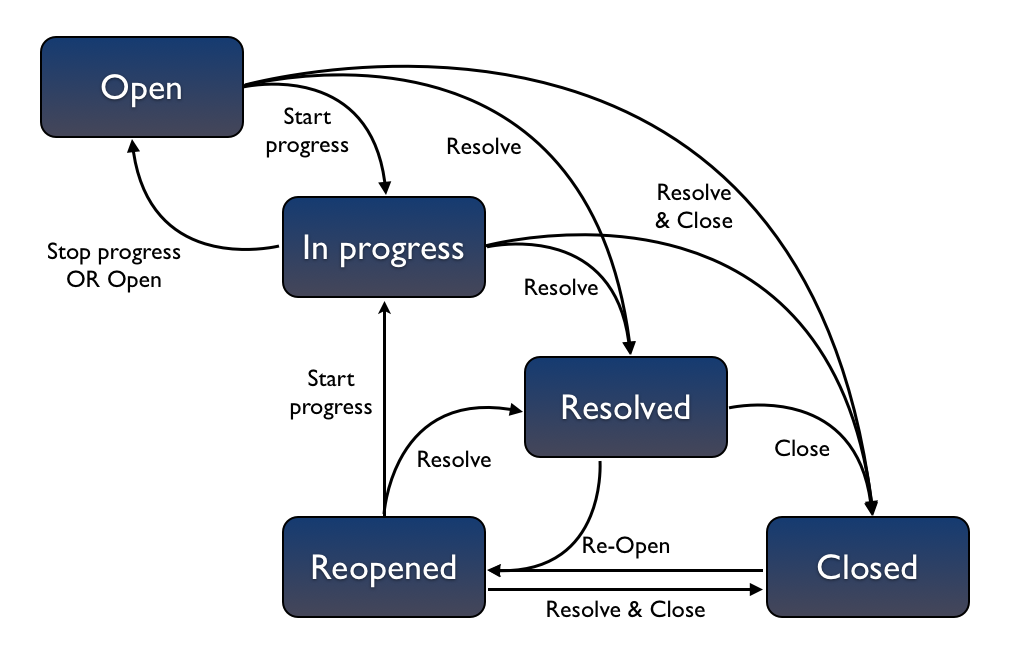
\includegraphics[width=0.6\textwidth]{jira-workflow.png}
\end{wrapfigure}

Une \textbf{étape} représente l'état courant du workflow pour une issue.
%% Chaque étape du workflow est liée à un état. 
Lorsqu'une issue est déplacée dans une étape particulière, son champ
\textit{status} est mis à jour et prend la valeur de l'état lié à l'étape.
Dans le diagramme ci-contre, les boîtes bleus représentent les étapes/états.

Une \textbf{transition} est un lien entre deux étapes. Une transition permet
à une issue de se déplacer d'une étape à une autre. Pour qu'une issue puisse
progresser depuis une étape particulière à une autre, une transition qui les
lie doit exister entre ces deux étapes.
Il faut noter qu'une transition est un lien unidirectionnel, donc si une
issue a besoin de faire des aller-retours entre deux étapes, deux
transitions doivent être créées.
Dans le diagramme ci-contre, les flèches représentent les transitions.

